\subsection{Descripción del algoritmo implementado.}
\vspace*{0.3cm}

La \textbf{heurística de búsqueda local} consiste en una heurística que
comienza con una solución dada que intentamos mejorar, progresivamente. Llamamos a esta solución ``candidata''. Luego, revisamos iterativamente sus soluciones ``vecinas''. Este conjunto de soluciones vecinas conforma el
\textit{espacio de búsqueda} y sus elementos son también potenciales soluciones candidatas. Esto sólo es posible si la vecindad contiene más elementos aparte de nuestra solución actual.

Si existe una mejor solución, se selecciona como solución actual y se repite el proceso, buscando en la vecindad de la nueva solución.

En particular, utilizamos una solución generada por la heurística golosa y verificamos mediante la búsqueda local si ésta es mejorable.

\vspace*{0.3cm}

Para nuestro algoritmo, planteamos las siguientes 2 estrategias para elegir vecindades:

\begin{itemize}
    \item \textbf{mover:} Una partición es vecina de otra si consiste en mover un único vértice de un conjunto a otro, es decir, $P$ y $Q$ son vecinas si existen $v \in A \in P$ y $B \in Q$ tales que $A - v = B$.

    \item \textbf{intercambiar:} Una partición es vecina de otra si consiste en intercambiar 2 vértices de distintos conjuntos, es decir, $P$ y $Q$ son vecinas si existen $v \in A \in P$ y $w \in B \in Q$ tales que $(A - v) \cup \{w\} = (B - w) \cup \{v\}$.
\end{itemize}

Los algoritmos consisten en, partiendo de una solución inicial, probar todas las soluciones vecinas y continuar desde la de menor peso. Cuando no se pueda mejorar más, finaliza la ejecución.

\vspace*{0.75cm}

\textbf{Pseudocódigo de la heurística mover:}

\vspace*{0.3cm}

\begin{verbatim}
mientras se pueda mejorar
  partición mínima =  mínimo peso(para cada vertice
                                    para cada conjunto excepto el del vertice
                                      mover vértice al conjunto)

  si peso partición mínima < peso actual
    intercambiar partición actual por la mínima
  sino
    ya no se puede mejorar
\end{verbatim}

\textbf{Pseudocódigo de la heurística intercambiar:}

\vspace*{0.3cm}

\begin{verbatim}
mientras se pueda mejorar
  partición mínima =  mínimo peso(para cada par de vértices
                                    intercambiar vértices)

  si peso partición mínima < peso actual
    intercambiar partición actual por la mínima
  sino
    ya no se puede mejorar
\end{verbatim}



\newpage
\subsection{Análisis de complejidad del peor caso de una iteración del
            algoritmo de búsqueda local.}
\vspace*{0.3cm}

Sea $G = (V,E)$ y consideremos $n = |V|$ y $m = |E|$.

La función \texttt{buscarConjunto} recorre todos los conjuntos y en cada uno
busca, en tiempo logarítmico, el vértice dado. Esta función realiza sobre cada
conjunto $O(\log(\text{cantidad de vértices del conjunto}))$ comparaciones,
realizadas en $O(1)$. A su vez, la cantidad de elementos de cada conjunto está
acotada por $n$. Luego, la complejidad de esta función es $O(k\log(n))$, siendo
$k$ el parámetro de entrada.

\vspace*{0.3cm}

En cada iteración, el algoritmo de búsqueda local con la estrategia de
\textit{mover} comienza a recorrer cada vértice del grafo, realizando lo siguiente:
\begin{itemize}
  \item Se llama a la función \texttt{buscarConjunto}, la cual pertenece a
  $O(k\log(n))$.

  \item Por cada conjunto de la partición, se calcula el peso obtenido al
  agregarlo al conjunto, llamando a la función \texttt{costo}. Al igual que en
  la función \texttt{agregarAlDeMenosPeso} explicada el análisis de complejidad del ejercicio 3, esto pertenece a $O(k + n)$.
\end{itemize}

Luego de recorrer cada vértice, se pueden llegar a realizar 2 llamados a
la función \texttt{costo}, que pertenece a $O(n)$.

Por lo tanto, en cada iteración del algoritmo de búsqueda local, la complejidad
es
\begin{center}
  $O(n (k\log(n) + k + n) + n) = O(nk\log(n) + nk + n^2 + n) = O(nk\log(n) +
n^2)$.
\end{center}

\vspace*{0.3cm}

En cada iteración, el algoritmo de búsqueda local con la estrategia de
intercambiar comienza a recorrer cada vértice del grafo, realizando lo siguiente:

\begin{itemize}
  \item Se llama a la función \texttt{buscarConjunto}, la cual pertenece a
  $O(k\log(n))$.

  \item Por cada uno de los otros vértices que no están en el mismo conjunto
  que el vértice actual:

  \begin{itemize}
    \item Se llama de nuevo a la función \texttt{buscarConjunto}.

    \item Se llama 4 veces a la función \texttt{costo}.
  \end{itemize}
\end{itemize}

Finalmente, se pueden llegar a realizar 4 llamados más a la función
\texttt{costo}.

Por lo tanto, en cada iteración del algoritmo de búsqueda local, la complejidad
es
\begin{center}
  $O(n (k\log(n) + n (k\log(n) + k + n)) + k + n)$.
\end{center}

\vspace{0.3cm}

Luego, la complejidad total del algoritmo pertenece a
\begin{center}
  $O(n^2k\log(n) + n^3)$.
\end{center}


\newpage \subsection{Experimentación y gráficos.}

\subsubsection{Tiempos de ejecución}

Para comparar los tiempos de ejecución, generamos diversos grafos de entrada
variando sus tamaños. Además, probamos con una solución inicial completamente
aleatoria y una generada por el algoritmo goloso.

\vspace*{0.75cm}

Variando la cantidad de vértices de un grafo denso (tomando $m$ para tener el
75\% de aristas de un grafo completo), a partir de la solución que devuelve el
algoritmo goloso. $n$ crece de a 20, comenzando en 20 y terminando en 500.  $k$
vale constantemente 10.

\vspace*{0.5cm}

\begin{figure}[H]
  \begin{center}
    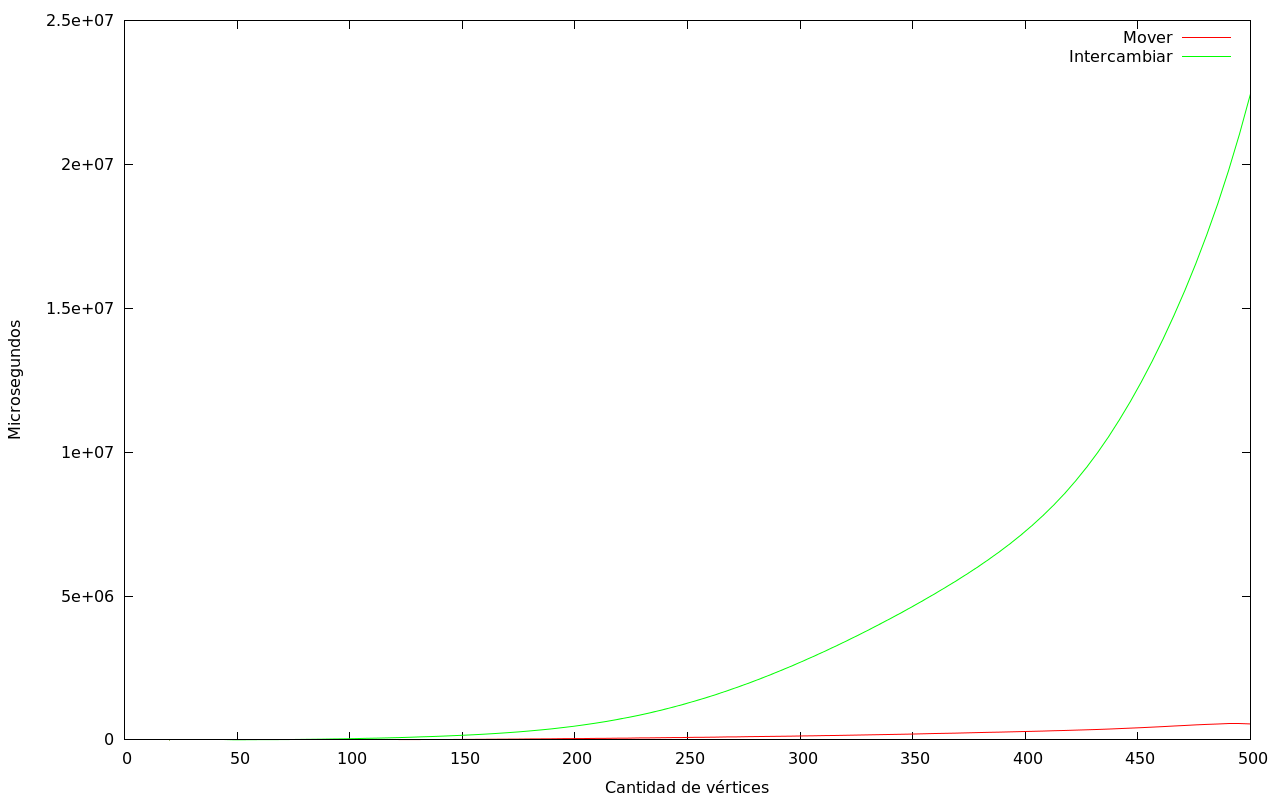
\includegraphics[scale=0.35]{imagenes/local-goloso-n-tiempo.png}
  \end{center}
\end{figure}

\newpage

Utilizando la misma configuración para $n$, $m$ y $k$, pero partiendo de una
posible solución elegida al azar.

\vspace*{0.35cm}

\begin{figure}[H]
  \begin{center}
    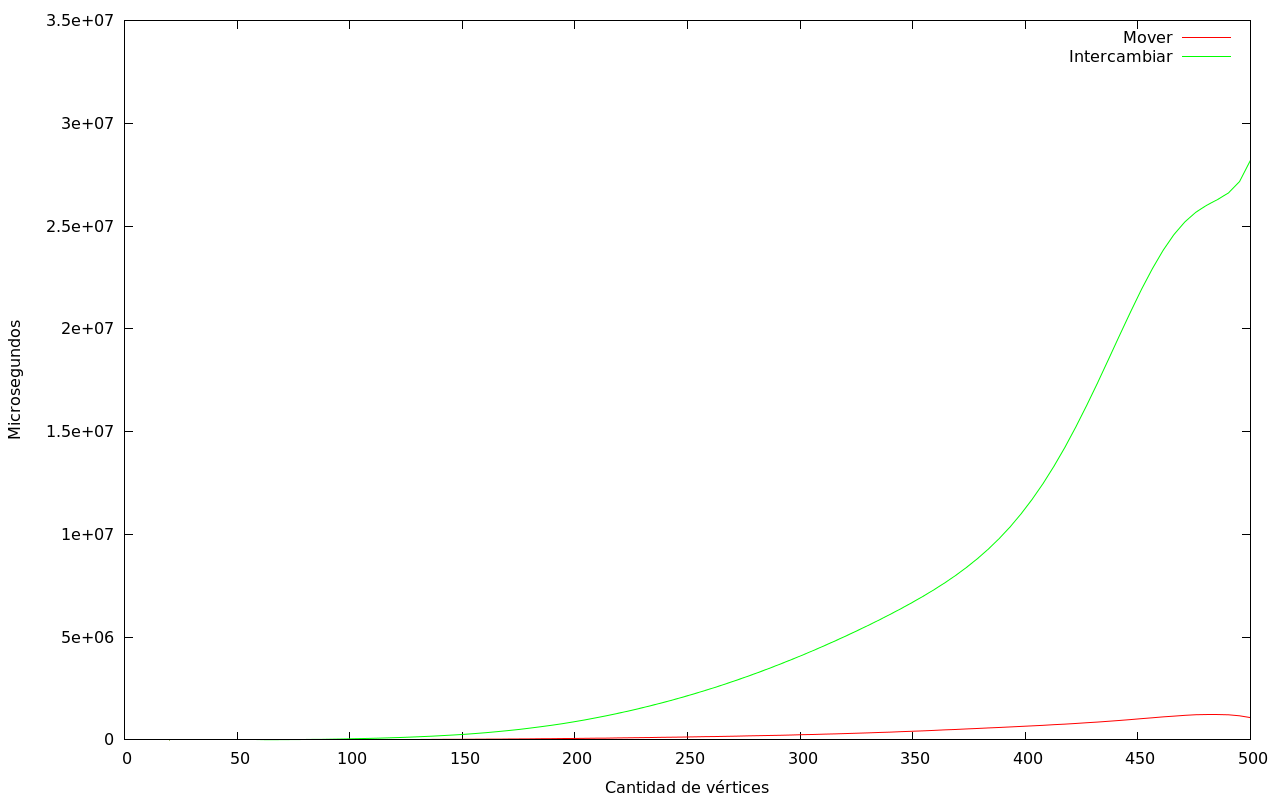
\includegraphics[scale=0.35]{imagenes/local-random-n-tiempo.png}
  \end{center}
\end{figure}

\vspace*{0.35cm}

Variando la cantidad de conjuntos de un grafo denso (200 vértices y 75\% de
aristas para un grafo completo), a partir de la solución que devuelve el
algoritmo goloso. $k$ aumenta de a 1, partiendo de 2, hasta 50.

\vspace*{0.5cm}

\begin{figure}[H]
  \begin{center}
    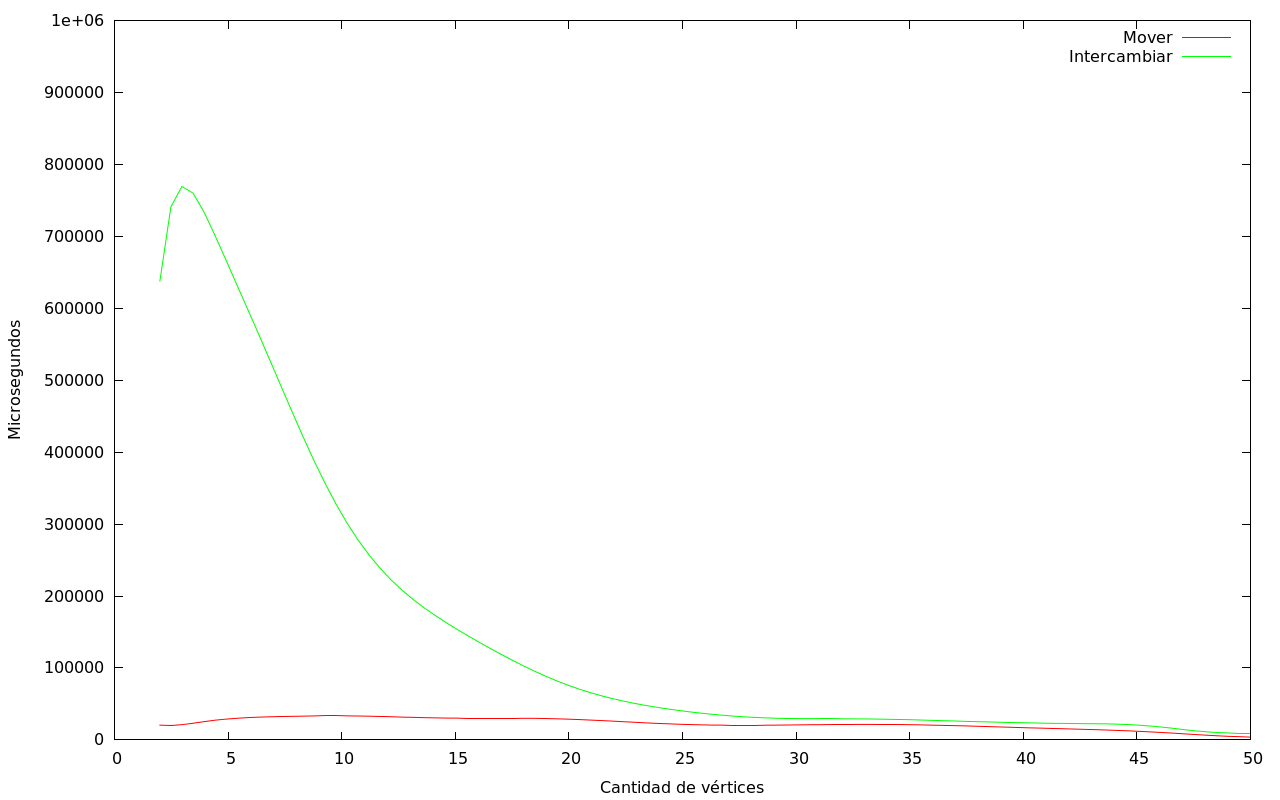
\includegraphics[scale=0.35]{imagenes/local-goloso-k-tiempo.png}
  \end{center}
\end{figure}

\vspace*{0.5cm}


Utilizando la misma configuración para $n$, $m$ y $k$, pero partiendo de una
posible solución elegida al azar.

\vspace*{0.5cm}

\begin{figure}[H]
  \begin{center}
    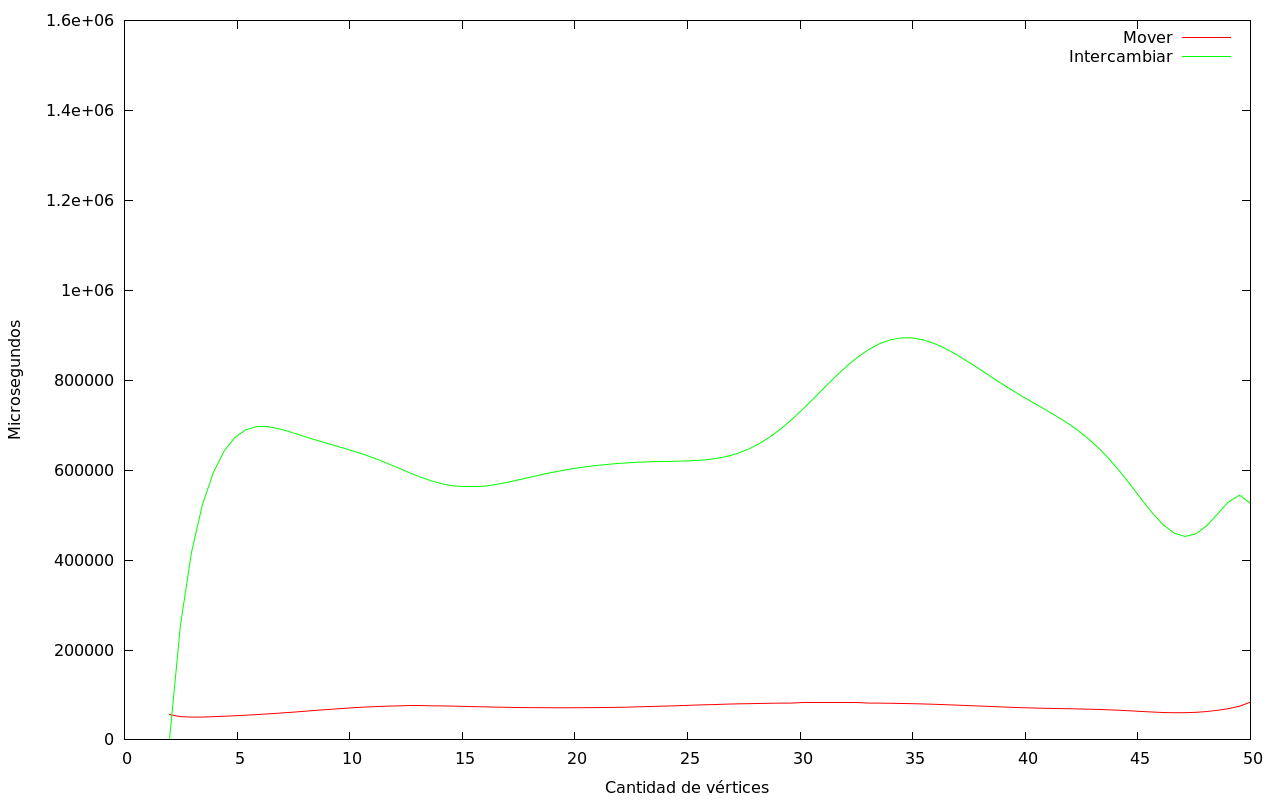
\includegraphics[scale=0.35]{imagenes/local-random-k-tiempo.png}
  \end{center}
\end{figure}

\vspace*{0.75cm}


Como puede observarse, en todos los casos el algoritmo de \textit{intercambiar}
es más lento que el algoritmo de \textit{mover}, cosa que era esperable,
considerando que \textit{intercambiar}, en cada iteración, tiene orden
$O(n^2k\log(n) + n^3)$, mientras que \textit{mover} tiene orden $O(nk\log(n) +
n^2)$.

También se puede apreciar que el tiempo crece (en ambos casos) cuando aumenta
el $n$, también razonable ya que la complejidad depende de éste.

Sin embargo, aunque podría esperarse que también aumente ligado al $k$, con una
solución al azar, el algoritmo \textit{mover} se mantiene constante y el
algoritmo \textit{intercambiar} varía mucho, aunque también acotado. No sucede
lo mismo cuando se comienza con la solución del goloso, que se comporta
de forma inversamente proporcional a $k$.

Esto seguramente se deba a que, con muchos conjuntos disponibles, la heurística golosa genera una solución muy cercana a la ideal. Luego, las heurísticas de búsqueda local necesitan ejecutarse pocas veces hasta encontrar un resultado que no pueda ser mejorado.


\newpage \subsubsection{Calidad}

Para comparar la calidad, observamos los pesos totales de la partición
utilizando las mismas variables que para comparar los tiempos de ejecución.

Un peso menor indica una solución de mejor calidad, queremos ver si alguna
de las dos heurísticas genera soluciones de mejor calidad, consistentemente.

\vspace{0.25cm}

Las configuraciones para $n$, $m$ y $k$ son las mismas que las utilizadas para
comparar tiempos: los dos primeros gráficos (1 y 2) corresponden a un grafo denso, donde varía $n$ y los dos últimos (3 y 4) a un grafo denso donde varía $k$.

\vspace*{0.75cm}

\textbf{Gráfico 1.}
\begin{figure}[H]
  \begin{center}
    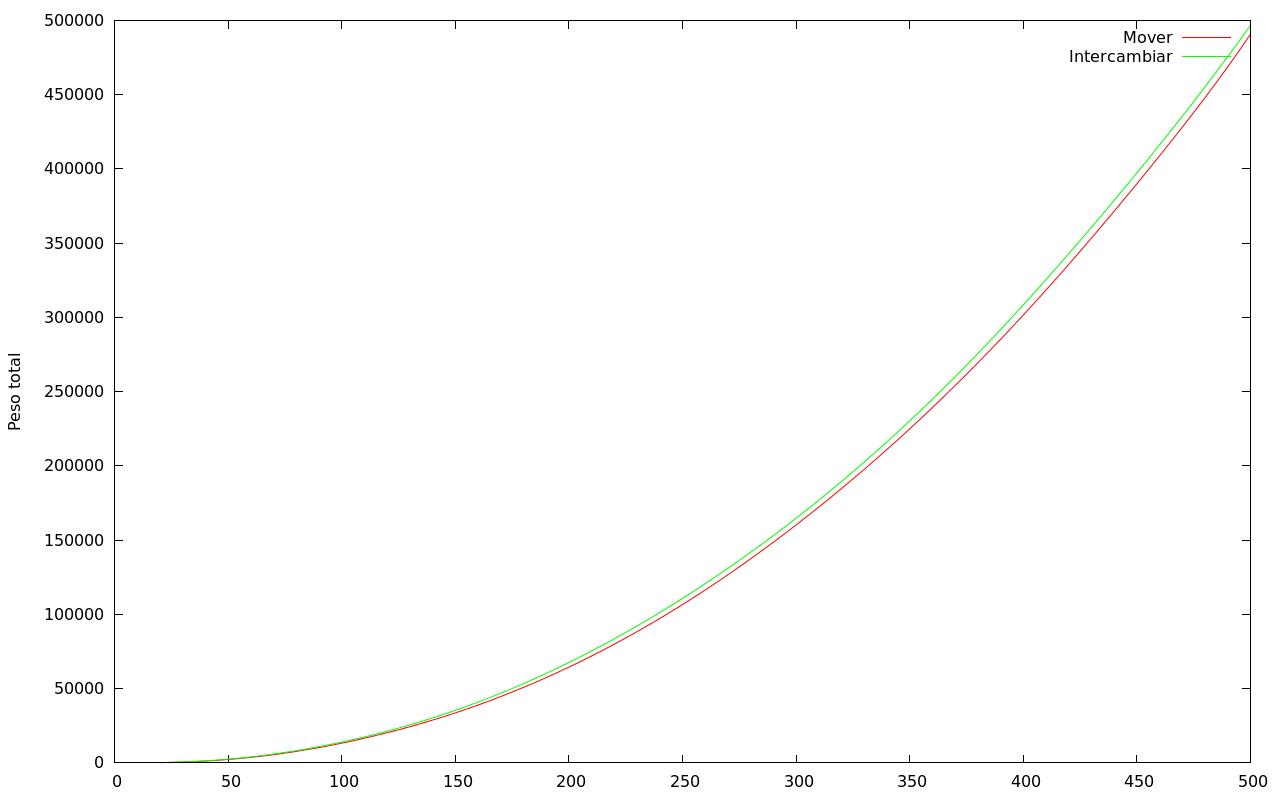
\includegraphics[scale=0.35]{imagenes/local-goloso-n-peso.png}
  \end{center}
\end{figure}

\newpage

\textbf{Gráfico 2.}
\begin{figure}[H]
  \begin{center}
    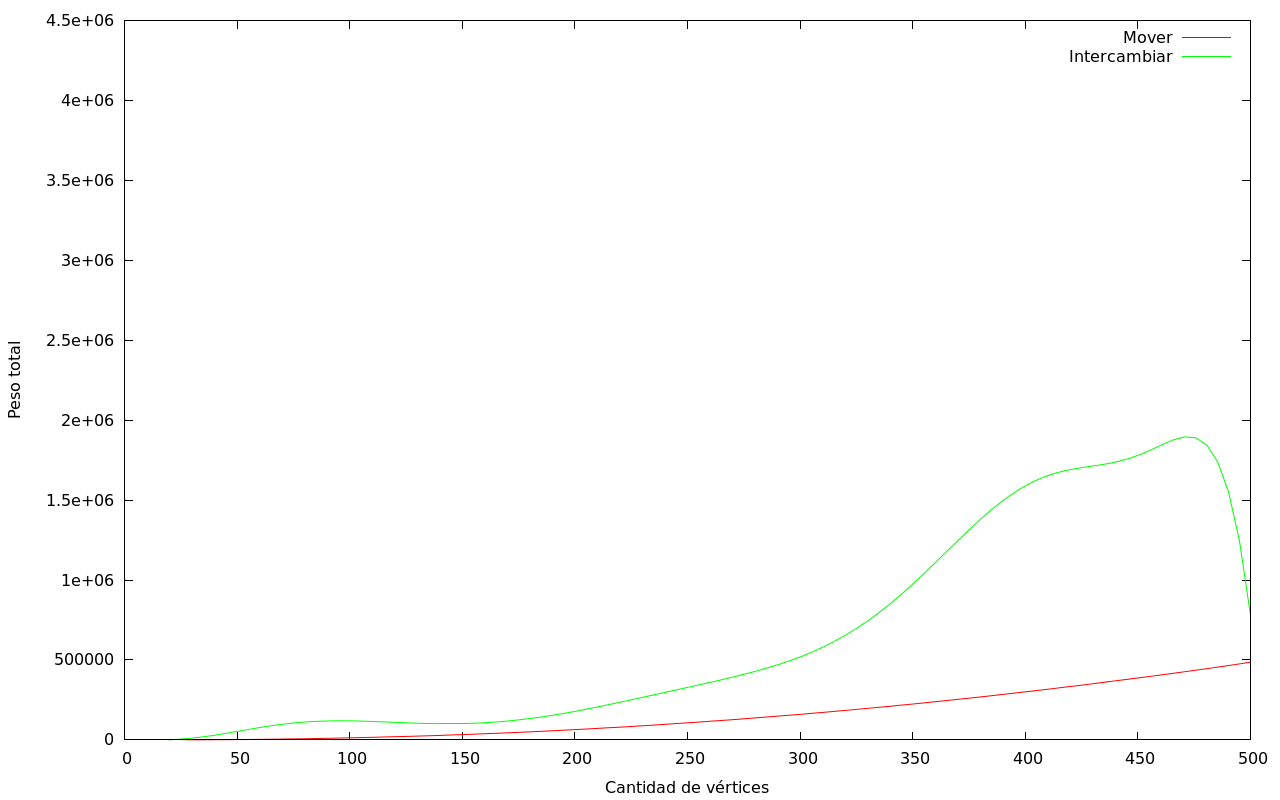
\includegraphics[scale=0.35]{imagenes/local-random-n-peso.png}
  \end{center}
\end{figure}

\vspace*{0.5cm}

\textbf{Gráfico 3.}
\begin{figure}[H]
  \begin{center}
    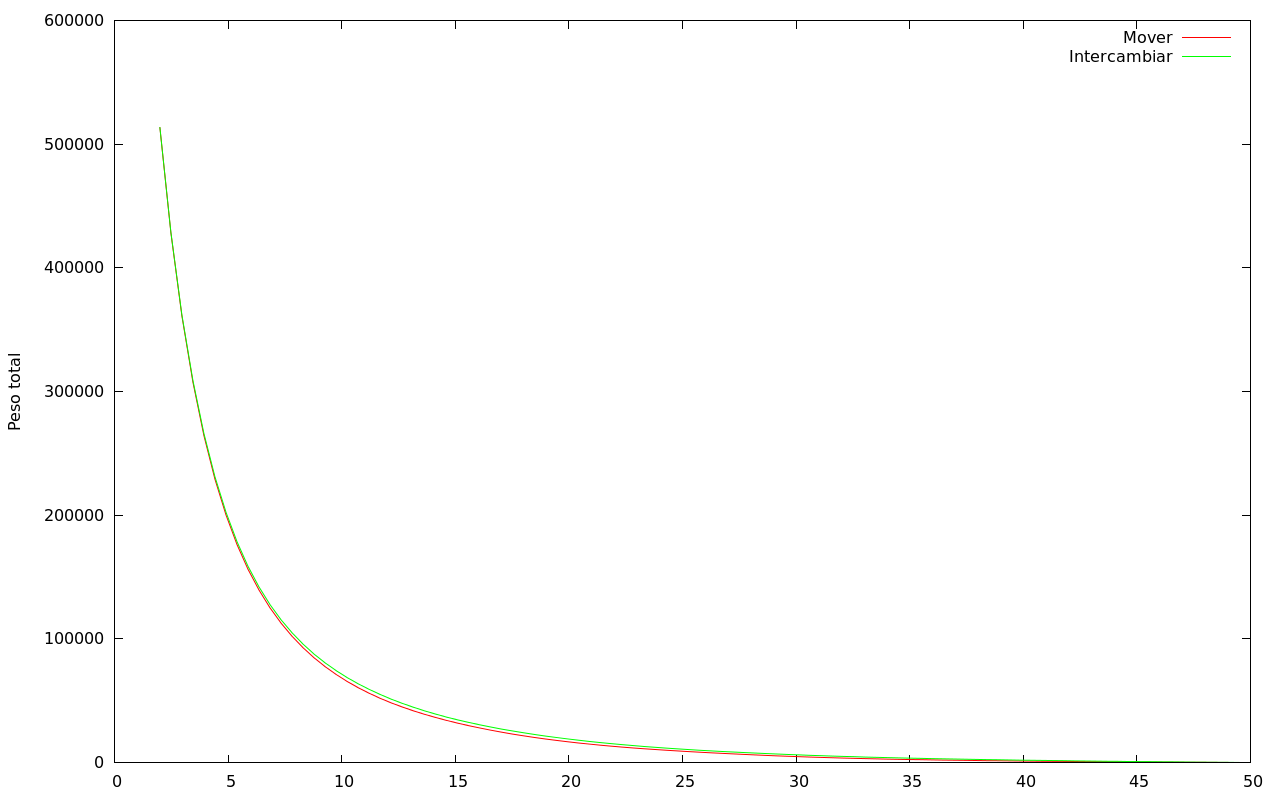
\includegraphics[scale=0.35]{imagenes/local-goloso-k-peso.png}
  \end{center}
\end{figure}

\newpage

\textbf{Gráfico 4.}
\begin{figure}[H]
  \begin{center}
    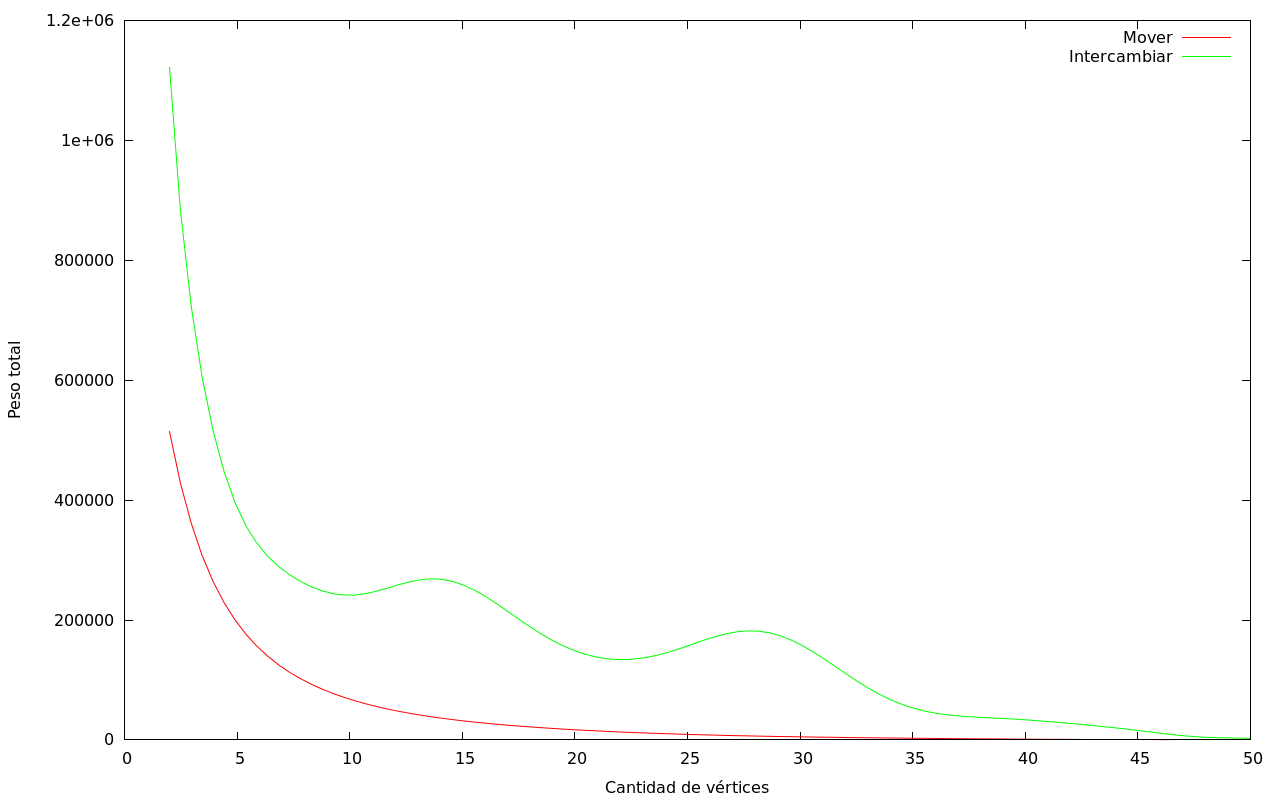
\includegraphics[scale=0.35]{imagenes/local-random-k-peso.png}
  \end{center}
\end{figure}

\vspace*{0.5cm}

Con estos gráficos, se puede observar que el algoritmo \textit{mover} genera
resultados de mejor calidad que el algoritmo \textit{intercambiar} para casi
todos los casos.

Variando la cantidad de vértices, el algoritmo \textit{mover} da resultados muy
similares empezando con la solución al azar tanto como con la solución generada
por el algoritmo goloso. Sin embargo, el algoritmo \textit{intercambiar}
encuentra una solución de calidad similar únicamente comenzando desde la
solución del goloso. Empezando desde la solución al azar, el peso crece mucho
más rápido que el peso del algoritmo \textit{mover}.

\vspace{0.25cm}

Algo similar encontramos al variar la cantidad de conjuntos. Cuando se comienza
desde una solución del goloso, se comportan de forma similar, pero empezando
con una solución aleatoria, el algoritmo \textit{intercambiar} no encuentra
buenas soluciones con la misma consistencia que el algoritmo \textit{mover}.

Luego de este análisis, con mejores tiempos y mejor calidad, queda muy evidente
que conviene utilizar la heurística de búsqueda local \textit{mover}.
